\chapter*{Hardware}
\addcontentsline{toc}{chapter}{Hardware}

\section*{Interrupt arbiter}
\addcontentsline{toc}{section}{Interrupt arbiter}

The arbiter has four states it can be in:

\begin{enumerate}
	\item \textbf{Zero} - the device does not require interrupts, or it does, but at the moment another device has not finished transmitting its interrupt request. In this state:

		If the device does not require an interrupt, then the IRQ and IAck pass through the arbiter from east to west and from west to east (it should be noted that if the processor is in the \textbf{WAITING} status, its raising of IAck is not considered as a response to the interrupt request, since being in this state, having received an interrupt request, the processor will only return to the \textbf{RUNNING} status, but will not process the request, the request will be processed after the transition to the \textbf{RUNNING} status)

		If the device requires an interrupt, but the other device has not finished transmitting its request, then the IAck output in the east cannot be raised again, but can be lowered (its high level indicates that the other device is transmitting its request)

		The transition from this state to the first is carried out provided that the device requires an interrupt and no other device is transmitting an interrupt request.
	\item The \textbf{first} is sending an interrupt request from the device.
		In this state:

		The IRQ to the west and IAck to the east are blocked, while the arbiter holds the IRQ output to the west at a high level, signaling the processor that an interrupt is required

		The transition from this state to the second is carried out provided that the processor has responded to the request by raising IAck (which means that the processor state allows the interrupt to be processed)
	\item \textbf{Second} - transfer of the interrupt vector to the processor
		In this state:

		The arbiter still holds the IRQ at a high level, since its lowering will lead to the termination of the interrupt request transfer process (unlike CdM-8, in which a fall in IRQ will cause a fall in IAck, which will trigger the interrupt vector latch in the processor, CdM-16 latches the interrupt vector on the falling edge of the clock, provided that there is an interrupt request and the necessary conditions inside the processor). In this case, the interrupt vector from the device is fed to the interrupt vector bus connected to the processor. Also, the raised IAck is transmitted to the device to notify it that the processor has responded to its request.

		The transition from this state back to zero and the completion of interrupt processing occurs on the falling edge of the clock, since it is at this moment that the processor latches the interrupt vector and the process of transmitting the request can be considered complete.
\end{enumerate}

\section*{Interrupt bus}
\addcontentsline{toc}{section}{Interrupt bus}

\begin{figure}[ht]
	\centering
	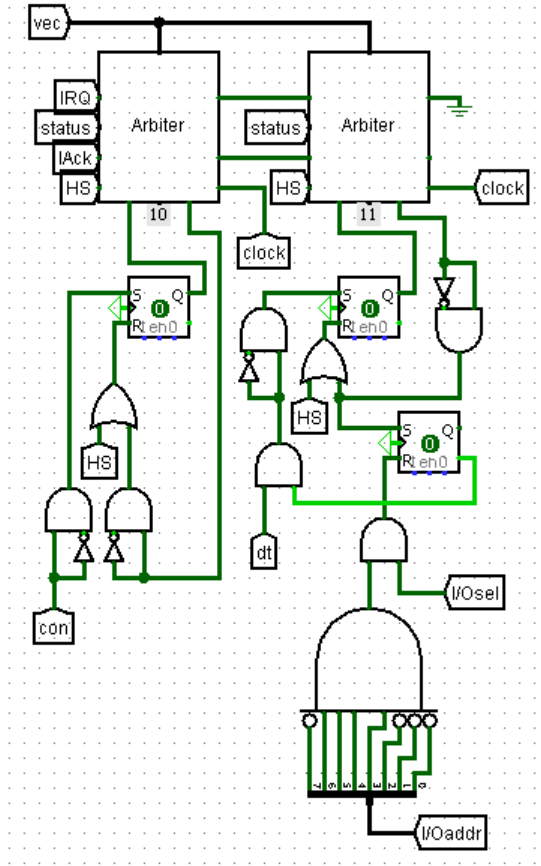
\includegraphics[scale=0.5]{intBus}
	\caption{Interrupt bus}
\end{figure}

Interrupt bus has two arbiters:

\begin{itemize}
	\item The first arbiter for outputting a greeting message. It has a higher priority and causes an interrupt when a remote terminal connects, sending a \textbf{con} signal.
	\item The second arbiter for processing commands. It has a lower priority and causes an interrupt when a command arrives in the UART buffer, sending a \textbf{dt} signal. In order to be able to process several commands that arrive one after another or one while the second is being read, a special address is used that sends a signal that the command reading has been completed.
\end{itemize}

\section*{Matrix controller}
\addcontentsline{toc}{section}{Matrix controller}

Matrix controller consist of two main parts:

\begin{itemize}
	\item Matrix buffer - main sequential unit, which stores current game field state and can be modified by processor or by game processor.
	\item Game processor - main combinatory unit, which calculates next field state based on current and on rules.
\end{itemize}

Other auxiliary devices, will be described later.

\subsection*{Matrix buffer row}
\addcontentsline{toc}{subsection}{Matrix buffer row}

\begin{figure}[ht]
	\centering
	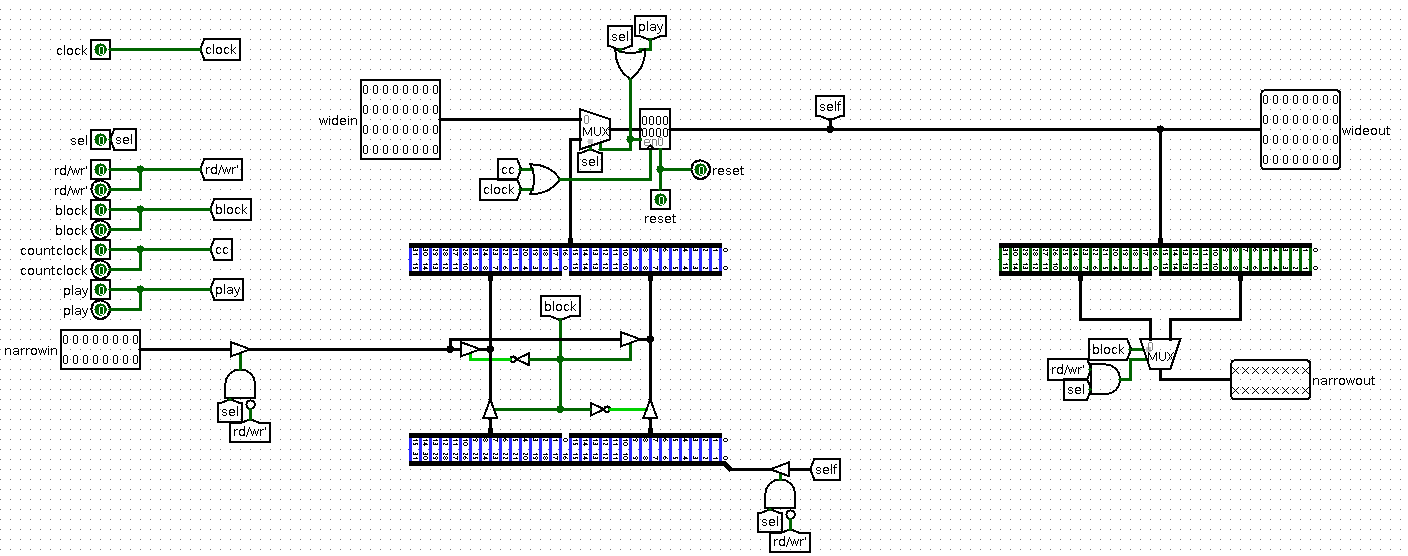
\includegraphics[width=\textwidth]{bufferRow}
	\caption{Buffer row}
\end{figure}

Here we have 32-bit register, holding state of one row of field and infrasctructure for modifying it and for reading its data. 

This register is enabled only if this row is \textbf{selected} as a distination of writing act of processor or if the game is \textbf{running}. Reasons of it is obvious, we don't need to change anything when the game paused and if processor isn't writing to this row.

Act of writing to this register can be triggered by rising edge of \textbf{clock} (so it will be synchronized with processor) or by rising edge of \textbf{cc} (counter clock) either (so it will be synchronized with game processor).

Also, because two sources of new state of this row (processor and game processor) changes different amount of bits in state at time (processor changes only first or second 16 bits of state due to size of data bus, game processor can change all 32 bits at time) there is two inputs in this circuit:

\begin{itemize}
	\item \textbf{Narrow in} - input from data bus of processor. This source is closed (by controlled buffer) when it's not needed (when there is no writing to this row from processor) same as \textbf{self} - current state of row, which needed for replacing one half of it while keeping another half unchanged (depends on \textbf{block} input, 0 - most significant bits, 1 - least significant bits).
	\item \textbf{Wide in} - input from game processor (new state of this row, calculated by game processor). This source goes straight to the multiplexer.
\end{itemize}

Which source of new state to use selects multiplexer in the west of register. It's disabled, when register is disabled, and when it's enabled, it selects source depend on \textbf{sel} input, if \textbf{sel} is high, this mean, that we need to take new state from processor, from \textbf{narrow in} combined with current state, when \textbf{sel} is low, we need to take new state from game processor, from \textbf{wide in}.

Respectively, in the east side of circuit we have two outputs:

\begin{itemize}
	\item \textbf{Narrow out} - output to data bus of processor. Row will pass its first or second half on this buss (depends on \textbf{block} again) if processor reads data from this row, otherwise it won't pass anything.
	\item \textbf{Wide out} - output to game processor. Row always pass its current state to let game processor calculate its new state if game is running.
\end{itemize}

Also, in the west side of circuit we can see, that some of inputs goes straight to output, named same as an input. This needed to pass some signals through all of rows, then they stay one above another (we will see it in next section).

This is how this circuit looks in other circuits:

\begin{figure}[ht]
	\centering
	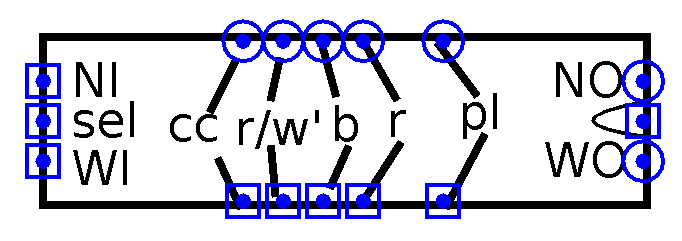
\includegraphics[scale=0.5]{bufferRowAppearence}
	\caption{Buffer row appearence}
\end{figure}

\clearpage

Here we have all of described inputs and outputs labeled.

\subsection*{Matrix buffer}
\addcontentsline{toc}{subsection}{Matrix buffer}

\begin{figure}[ht]
	\centering
	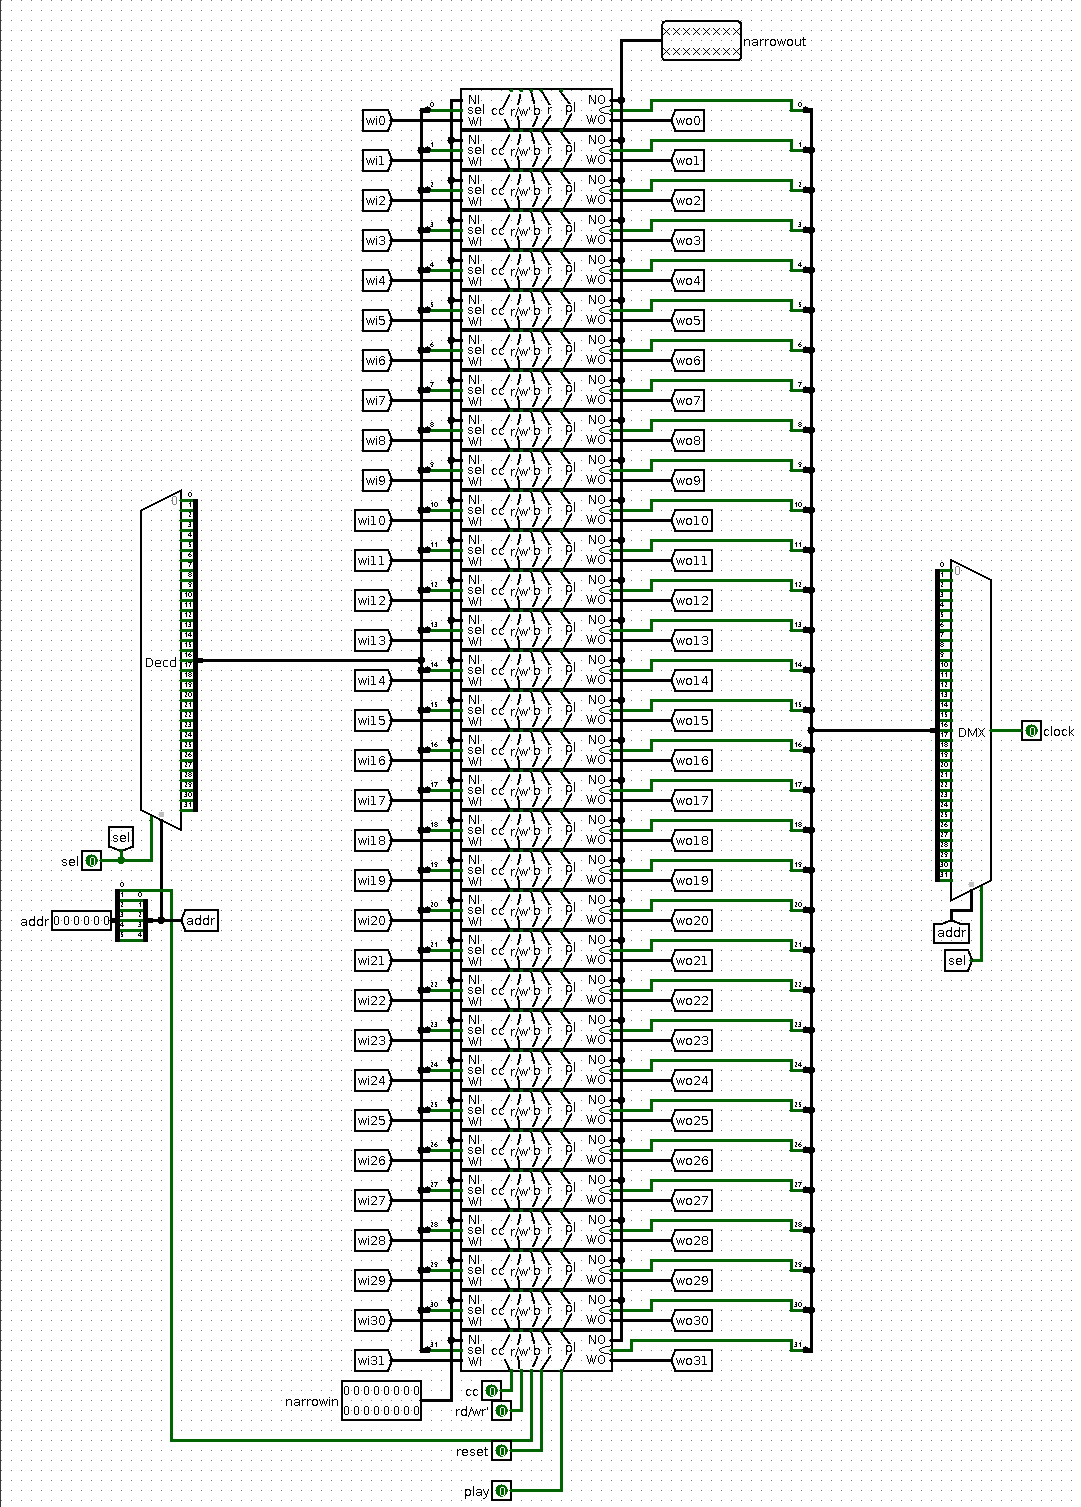
\includegraphics[scale=0.5]{buffer}
	\caption{Matrix buffer}
\end{figure}

Here we have 32 \textbf{matrix buffer rows}, connected with each other in one big block - matrix buffer. All \textbf{narrow ins} connected to one narrow in input in the south of circuit, which connected to data bus. Also, all \textbf{narrow outs} connected to one narrow out output, connected to data bus.

Where is decoder for selecting appropriate row by address and demultiplexer to pass clock signal only to the row, which selected.

All of wide inputs connected to 32 separate 32 bit inputs and all of wide outputs connected to 32 separate 32 bit outputs.

\clearpage
Here is matrix buffer appearence:

\begin{figure}[ht]
	\centering
	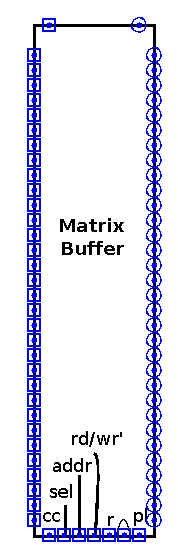
\includegraphics[scale=0.5]{bufferAppearence}
	\caption{Matrix buffer appearence}
\end{figure}

\subsection*{Cell}
\addcontentsline{toc}{subsection}{Cell}

\begin{figure}[!htb]
	\centering
	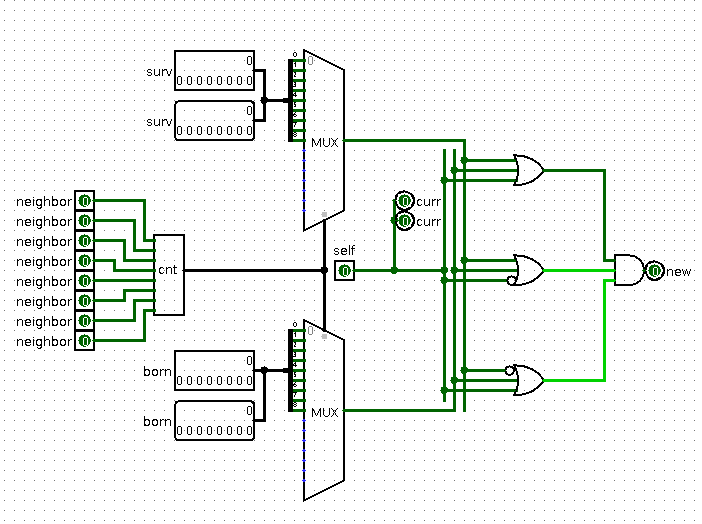
\includegraphics[scale=0.3]{cell}
	\caption{Cell}
\end{figure}

Cell is a single calculator, which calculates new state of single cell, based on its neighbours (actually on amount of alive neighbours), current status of cell and rules.

This is done by two multiplexers, selecting if cell should survive or should it become alive, and CNF, which represents following truth table:

\begin{center}
	\begin{tabular}{|c|c|c|c|}
		\hline
		Surv & Born & State & New \\
		\hline
		0 & 0 & 0 & 0  \\
		\hline
		0 & 0 & 1 & 0 \\
		\hline
		0 & 1 & 0 & 1 \\
		\hline
		0 & 1 & 1 & 1 \\
		\hline
		1 & 0 & 0 & 0 \\
		\hline
		1 & 0 & 1 & 1 \\
		\hline
		1 & 1 & 0 & 1 \\
		\hline
		1 & 1 & 1 & 1 \\
		\hline
	\end{tabular}
\end{center}

\subsubsection*{Counter}
\addcontentsline{toc}{subsubsection}{Counter}

Circuit in the west side is counter, simple circuit which counts amount of its high inputs:

\begin{figure}[ht]
	\centering
	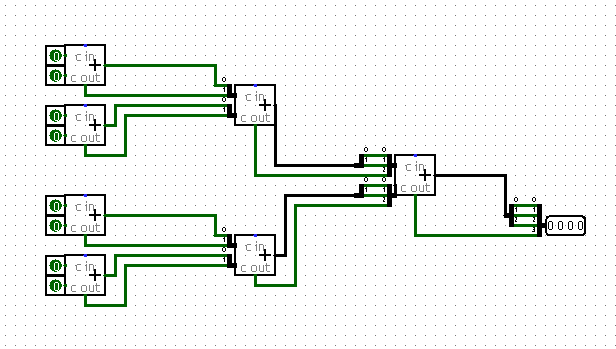
\includegraphics[scale=0.5]{counter}
	\caption{Counter}
\end{figure}

\subsection*{Game processor row}
\addcontentsline{toc}{subsection}{Game processor row}

\begin{figure}[ht]
	\centering
	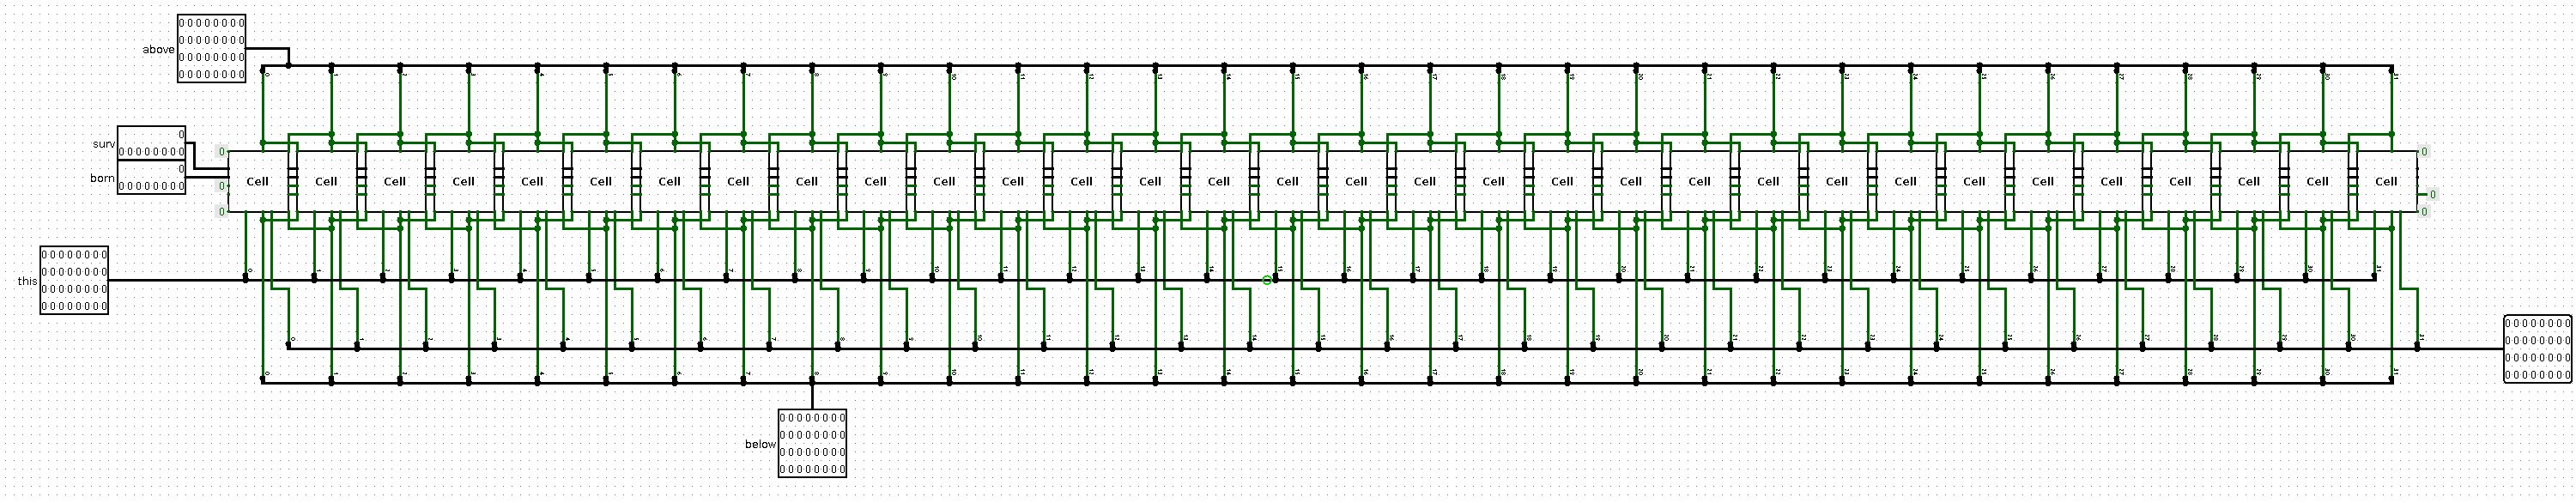
\includegraphics[width=\textwidth]{gameProcessorRow}
	\caption{Game processor row}
\end{figure}

This circuit is just 32 cells connected with each other in one row. This circuit have 3 inputs for rows:

\begin{enumerate}
	\item Row \textbf{above} this
	\item Row \textbf{below} this
	\item \textbf{This} row
\end{enumerate}

All of this inputs is \textbf{current} state of this rows.
Also, there is 2 inputs for rules, mentioned before: \textbf{surv} and \textbf{born}.

All of cells 8 \textbf{neighbour} inputs connected to appropriate wires with their neighbours statuses (except leftmost and rightmost cells, which don't have neighbours on the left and on the right respectively).

All of calculated \textbf{new} states of cells goes in single 32 bit wide wire, which goes to the only one output of game processor row - \textbf{new state of this row}.

Here is appearence of game processor row:

\begin{figure}[ht]
	\centering
	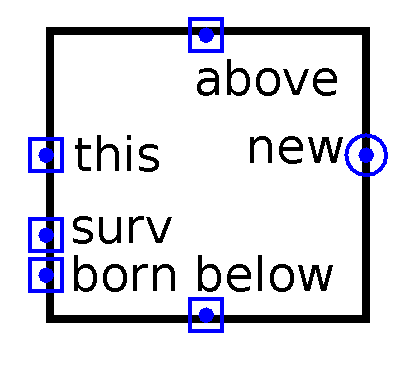
\includegraphics[scale=0.5]{gameProcessorRowAppearence}
	\caption{Game processor row appearence}
\end{figure}

\subsection*{Game processor}
\addcontentsline{toc}{subsection}{Game processor}

\begin{figure}[ht]
	\centering
	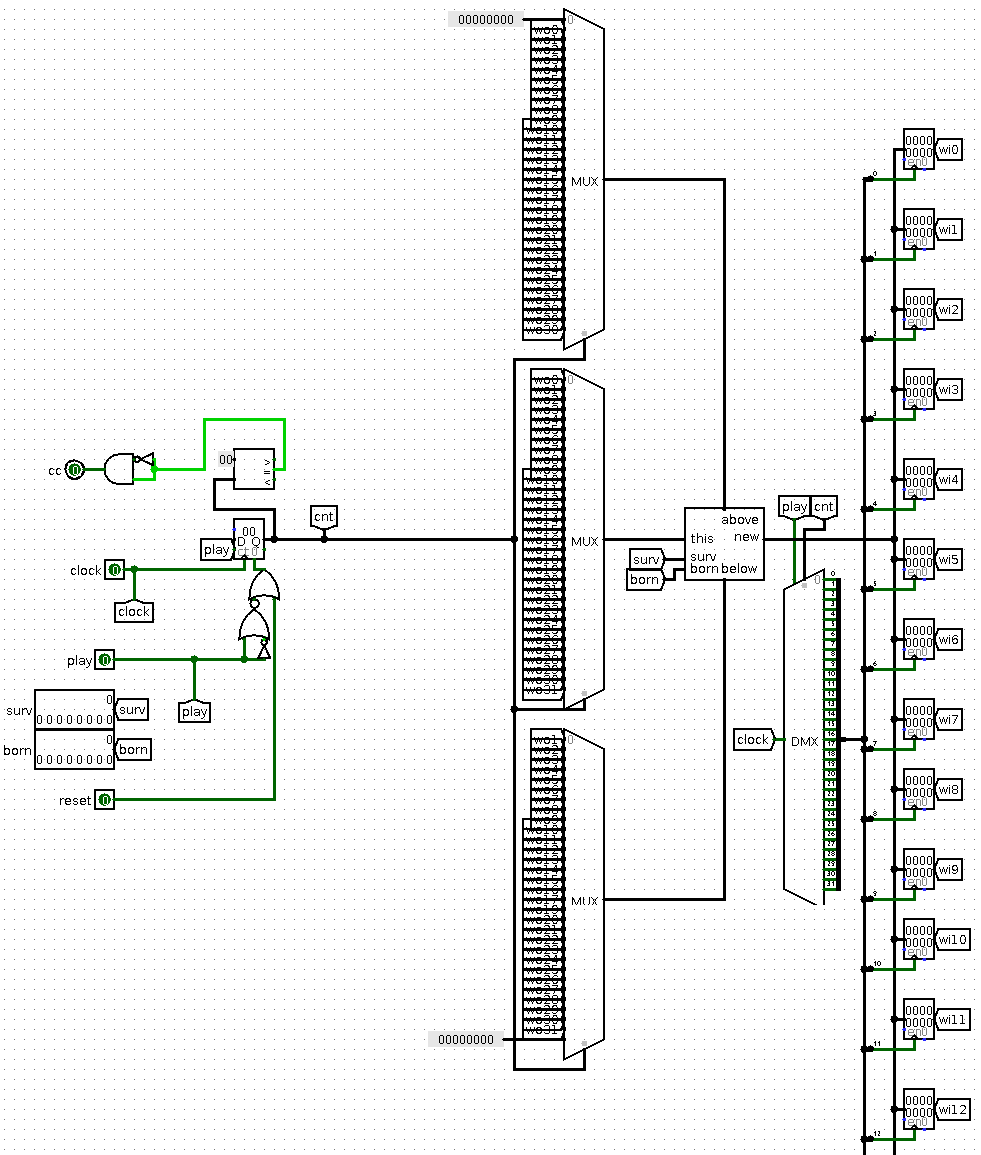
\includegraphics[scale=0.5]{gameProcessor}
	\caption{Game processor}
\end{figure}

Game processors purpose is to calculate new state of whole game field. New state is calculated, base on current, row by row. This is implemented by 32 bit counter, which indicates, which row will be calculated on this tick, and 3 multiplexers choosing appropriate \textbf{this} row, \textbf{above} row and \textbf{below} row for \textbf{game processor row} and 32 "buffering" registers, holding new state until it will be latched in matrix buffer.

Transition of counter value from 31 to 0 meaning, what all 32 row were calculated, causes rising of "equal" out of comparator (which compares counter value and 0), this triggers impulse on \textbf{cc} output and results in matrix buffer latching new state of whole game field.

Also, when game pauses, counter resets to zero, because we need to recalculate whole new game field state after (maybe) something will be changed when game is paused. 

\clearpage
\subsection*{Speed controller}
\addcontentsline{toc}{subsection}{Speed controller}

\begin{figure}[ht]
	\centering
	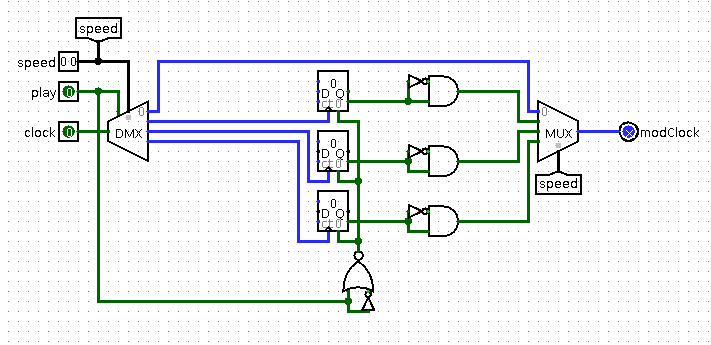
\includegraphics[scale=0.5]{speedController}
	\caption{Speed controller}
\end{figure}

This simple circuit stays for regulating speed of game. When game is running it will choose the way, through which clock will go depends on speed input:

\begin{itemize}
	\item Directly 
	\item Through counter, which (with rising edge detector, connected to carry output of counter) generates impulse every 2 ticks
	\item Through counter, which generates impulse every 4 ticks
	\item Through counter which generates impulse every 8 ticks
\end{itemize}

\subsection*{Status register}
\addcontentsline{toc}{subsection}{Status register}

\subsection*{One iteration trigger}
\addcontentsline{toc}{subsection}{One iteration trigger}

\section*{UART controller}
\addcontentsline{toc}{section}{UART controller}

\begin{figure}[ht]
	\centering
	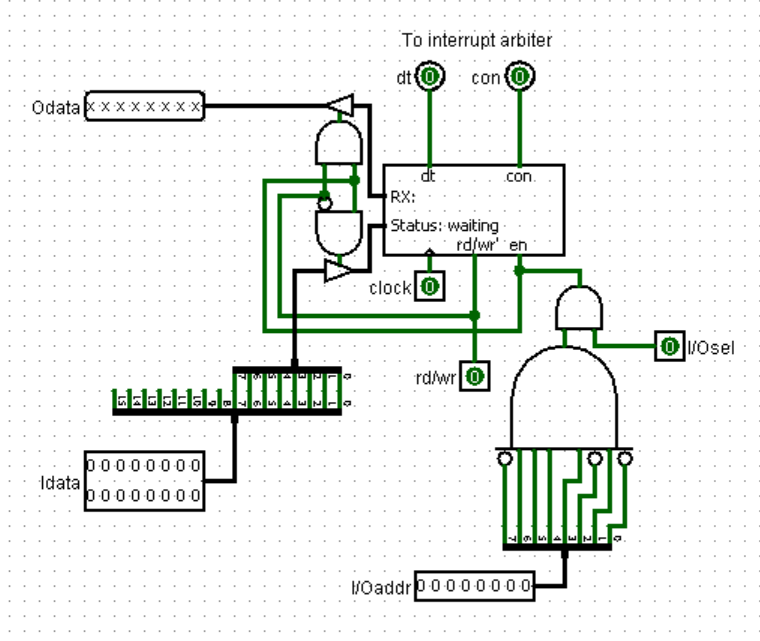
\includegraphics[scale=0.5]{uartController}
	\caption{UART controller}
\end{figure}

UART controller contains UART and I/O implementation.

\begin{itemize}
	\item When the processor accesses an address allocated in memory, it writes a character to the UARTa buffer via the data bus or retrieves it from there via the data bus depending on the rd/wr signal.
	\item UART raises the \textbf{dt} signal if a character arrives in the buffer, and the \textbf{con} signal if a remote terminal is connected to the UART.
\end{itemize}
